\documentclass{article}

% If neurips_2024.sty is available (recommended on Overleaf), uncomment one line below.
% \usepackage[preprint]{neurips_2024}
% \usepackage[final]{neurips_2024}

\usepackage[utf8]{inputenc}
\usepackage[T1]{fontenc}
\usepackage{hyperref}
\usepackage{url}
\usepackage{booktabs}
\usepackage{amsfonts}
\usepackage{nicefrac}
\usepackage[numbers]{natbib}
\usepackage{microtype}
\usepackage{xcolor}
\usepackage{graphicx}
\usepackage{amsmath,amssymb}

\title{Symmetry-Aware PPO for Quadrotor Hover Control: Interim Empirical Study}

\author{
  SS26 Drone Control Team \\
  MetaRL Project \\
  \texttt{internal-report@metarl.local}
}

\begin{document}

\maketitle

\begin{abstract}
This interim report summarizes symmetry-aware reinforcement learning experiments for quadrotor hover control. We compare baseline PPO, augmentation-only variants, mirror-loss variants, and a discretized yaw-augmentation family ($C_n$). We aggregate results from TensorBoard logs using the mean of the final 50 \texttt{Train/mean\_reward} points per run. Augmentation-only variants provide the best performance and stability so far, while the discretized-$C_n$ ablation indicates strongest results around $n\in\{6,8\}$.
\end{abstract}

\section{Introduction}
Quadrotor policy learning can be sensitive to observation transformations and action-space symmetries. Symmetry-aware RL introduces inductive structure through equivariant augmentation and consistency objectives, often improving optimization stability and sample efficiency~\citep{mukhopadhyay2020survey,sanchez2023symmetric}. This report summarizes current project results for symmetry-aware PPO on hover control.

\section{Setup}
\paragraph{Environment and algorithm.}
We train PPO in a direct RL quadrotor hover task with velocity regularization and distance-to-goal tracking terms.

\paragraph{Compared variants.}
\begin{itemize}
    \item \textbf{baselines}: standard PPO.
    \item \textbf{aug\_only}: symmetry augmentation only.
    \item \textbf{aug\_only\_c4}: fixed $C_4$ augmentation.
    \item \textbf{mirror\_loss\_only}: mirror loss only.
    \item \textbf{aug\_plus\_mirror\_loss}: augmentation + mirror loss.
    \item \textbf{aug\_mirror}: historical combined family in logs.
\end{itemize}

\paragraph{Metric.}
For each run, we compute
\begin{equation}
R_{\mathrm{final}} = \frac{1}{K}\sum_{i=1}^{K} r_i, \quad K=\min(50, N_{\mathrm{logged}}),
\end{equation}
where $r_i$ are the final scalar values of \texttt{Train/mean\_reward}. Tables report mean and standard deviation across runs.

\section{Yaw Equivariance with Discretization}
We model yaw symmetry as the action of the cyclic group $C_n\subset SO(2)$ on state-action space.
Define the planar rotation
\begin{equation}
R(\theta)=
\begin{bmatrix}
\cos\theta & -\sin\theta\\
\sin\theta & \cos\theta
\end{bmatrix},
\quad
\theta_k=\frac{2\pi k}{n},\;k\in\{0,\ldots,n-1\}.
\end{equation}

The policy observation and action are
\begin{equation}
s=[v_x,v_y,v_z,\omega_x,\omega_y,\omega_z,g_x,g_y,g_z,d_x,d_y,d_z]^{\top},
\end{equation}
\begin{equation}
a=\begin{bmatrix}T&m_x&m_y&m_z\end{bmatrix}^{\top}.
\end{equation}

For each $\theta\in C_n$, define state and action transforms
\begin{equation}
s'=T_s(\theta)s,\qquad a'=T_a(\theta)a,
\end{equation}
with component-wise action
\begin{equation}
\begin{aligned}
\begin{bmatrix}v'_x\\v'_y\end{bmatrix} &= R(\theta)\begin{bmatrix}v_x\\v_y\end{bmatrix},
\begin{bmatrix}\omega'_x\\\omega'_y\end{bmatrix} = R(\theta)\begin{bmatrix}\omega_x\\\omega_y\end{bmatrix},\\
\begin{bmatrix}g'_x\\g'_y\end{bmatrix} &= R(\theta)\begin{bmatrix}g_x\\g_y\end{bmatrix},
\begin{bmatrix}d'_x\\d'_y\end{bmatrix} = R(\theta)\begin{bmatrix}d_x\\d_y\end{bmatrix},
\end{aligned}
\end{equation}
and invariant channels
\begin{equation}
v'_z=v_z,\quad \omega'_z=\omega_z,\quad g'_z=g_z,\quad d'_z=d_z.
\end{equation}
For actions, thrust and yaw moment are invariant, while in-plane moments rotate:
\begin{equation}
T'=T,\quad m'_z=m_z,\quad
\begin{bmatrix}m'_x\\m'_y\end{bmatrix}=R(\theta)\begin{bmatrix}m_x\\m_y\end{bmatrix}.
\end{equation}

Given a mini-batch $\mathcal{B}=\{(s_i,a_i)\}_{i=1}^{B}$, discretized augmentation is
\begin{equation}
\mathcal{A}_{C_n}(\mathcal{B})=
\bigcup_{k=0}^{n-1}
\{(T_s(\theta_k)s_i,\,T_a(\theta_k)a_i)\}_{i=1}^{B},
\end{equation}
which yields an $nB$-sample batch. In implementation, this is realized as the original batch ($k=0$) plus $n-1$ rotated copies.

The target symmetry property is policy equivariance:
\begin{equation}
\pi\!\left(T_s(\theta)s\right)=T_a(\theta)\pi(s),\qquad \forall\theta\in C_n,
\end{equation}
approximated here via data augmentation during PPO updates.

\section{Results}
\subsection{Family-level comparison}
\begin{table}[t]
\caption{Final reward summary by experiment family.}
\label{tab:family}
\centering
\begin{tabular}{lrrrrr}
\toprule
Family & Runs & Mean & Std & Min & Max \\
\midrule
baselines & 11 & 127.11 & 4.60 & 117.06 & 132.31 \\
aug\_only & 11 & 131.41 & 2.26 & 125.71 & 133.97 \\
aug\_only\_c4 & 11 & 131.30 & 1.59 & 127.28 & 132.66 \\
mirror\_loss\_only & 3 & 124.44 & 4.59 & 118.61 & 129.82 \\
aug\_plus\_mirror\_loss & 3 & 127.43 & 3.15 & 123.32 & 130.96 \\
aug\_mirror & 12 & 122.74 & 13.42 & 98.85 & 133.97 \\
\bottomrule
\end{tabular}
\end{table}

Augmentation-only variants improve over baseline by about 4.2 reward points on average and show reduced variance.

\subsection{$C_n$ discretization ablation}
The new discretized yaw experiments under \texttt{aug\_only\_theta} compare $C_4$, $C_6$, $C_8$, and $C_{12}$.

\begin{table}[t]
\caption{$C_n$ ablation (3 runs per class).}
\label{tab:cn}
\centering
\begin{tabular}{lrrrrr}
\toprule
Class & Runs & Mean & Std & Min & Max \\
\midrule
$C_4$ & 3 & 130.85 & 1.05 & 129.36 & 131.65 \\
$C_6$ & 3 & 131.29 & 0.41 & 130.73 & 131.70 \\
$C_8$ & 3 & 131.28 & 1.25 & 130.02 & 132.98 \\
$C_{12}$ & 3 & 126.90 & 2.84 & 123.36 & 130.33 \\
\bottomrule
\end{tabular}
\end{table}

Current evidence indicates best performance in the moderate discretization regime ($n=6$ or $8$), while $C_{12}$ underperforms and is less stable.

\begin{figure}[t]
    \centering
    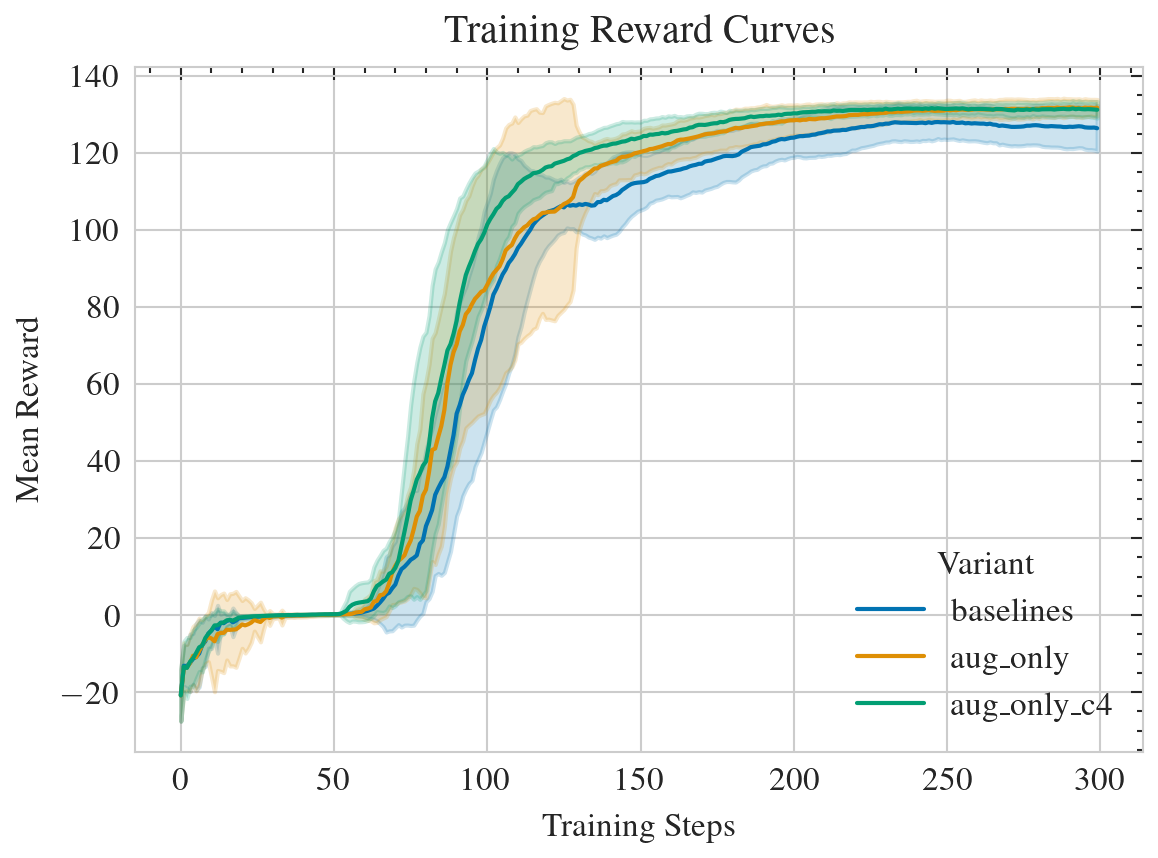
\includegraphics[width=0.98\linewidth]{figures/training_reward_curves.png}
    \caption{Training reward curves for baseline and symmetry families.}
    \label{fig:maincurves}
\end{figure}

\begin{figure}[t]
    \centering
    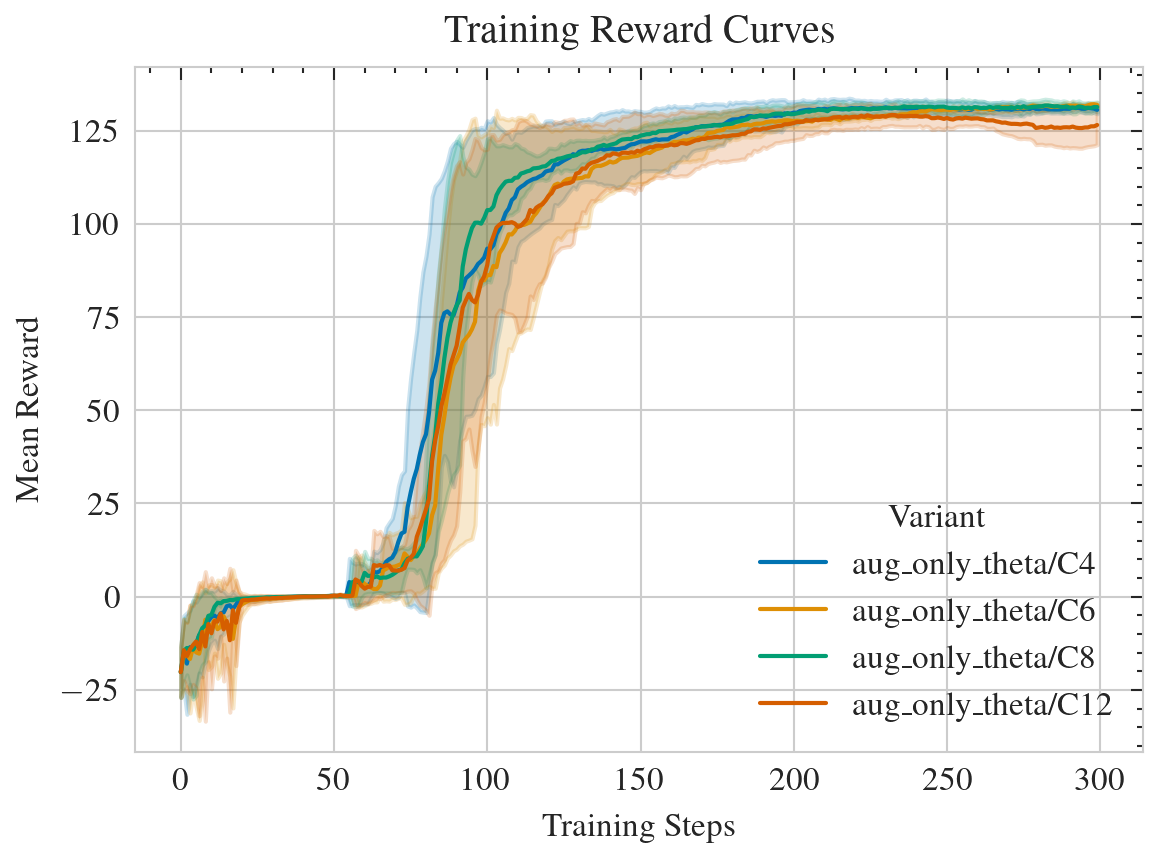
\includegraphics[width=0.98\linewidth]{figures/training_reward_curves_Cn.png}
    \caption{Training reward curves for discretized yaw classes ($C_n$).}
    \label{fig:cncurves}
\end{figure}

\section{Discussion and Next Steps}
Symmetry augmentation consistently improves training outcomes over baseline PPO in current experiments. Mirror-loss-focused variants are currently weaker, motivating additional coefficient and schedule tuning.

Planned next steps:
\begin{itemize}
    \item Increase $C_n$ seeds to at least 10 per class.
    \item Run matched-budget sweeps for $n\in\{4,6,8,10\}$.
    \item Re-evaluate mirror loss under stronger augmentation baselines.
    \item Add evaluation metrics beyond training reward (goal error and recovery behavior).
\end{itemize}

\section*{Acknowledgments}
This manuscript is an interim internal report generated from in-repo logs and plots.

\bibliographystyle{plainnat}
\bibliography{references}

\end{document}
